% Provenance (never printed): see sources/outline_sources.md (Year 3:
% geophysical fluid dynamics: rotating-frame equations, Rossby number,
% hydrostatic and geostrophic balance, thermal wind, buoyancy frequency).
% Brief: sources/book5/BRIEFS.md, ch. 19. Curves from
% figdata/bachelor-3/inertial_oscillation.py, thermal_wind.py and
% buoyancy_frequency.py. Exercise and problem values in the Book 5 scratch
% calculator calc/ch19.py. The Steppe of Orrin, its lake, its stations and
% its winds are invented.
\chapter{Dynamique des fluides géophysiques}\label{ch:b3:gfd-foundations}

Si l'on remue une tasse de thé, le tourbillon s'éteint en une minute~; les feuilles se rassemblent au
milieu du fond, et rien d'autre ne se passe. L'océan et l'atmosphère
sont brassés eux aussi, par le Soleil et le vent, mais sur une planète en rotation et dans
des couches de densités différentes. La rotation et la stratification les soumettent
à des règles qu'une tasse de thé ne laisse jamais voir~: les vents soufflent le long des
isobares plutôt qu'à travers, les colonnes de fluide refusent de s'incliner, et le vent de la
haute troposphère s'inscrit dans les températures situées en dessous. Ce chapitre pose les
équations de ces écoulements vastes, lents et minces, ainsi que les quelques nombres qui
déterminent quels termes comptent.

\begin{recall}
Les forces de Coriolis et centrifuge dans un référentiel tournant, les équations de Navier--Stokes
et de continuité, la viscosité, le nombre de Reynolds et la relation hydrostatique
sont dans les volumes de physique. Le paramètre de Coriolis $f = 2\Omega
\sin\varphi$, la force de gradient de pression, l'équilibre géostrophique, le
vent géostrophique et le \omterm{def:b3:gfd-foundations:gradient}{vent du gradient}, ainsi que les courants-jets, figurent dans le volume de première
année, dans son chapitre sur la circulation générale de l'atmosphère~; la couche
d'Ekman dans son chapitre sur la circulation de l'océan~; la température
potentielle, la stabilité statique et l'oscillation d'une parcelle d'air soulevée dans
son chapitre sur la structure de l'atmosphère et de l'océan.
\end{recall}

\section{Équations dans un référentiel tournant}\label{sec:b3:gfd-foundations:equations}

Dans un référentiel qui tourne avec la Terre à la vitesse angulaire
$\vec\Omega$, une parcelle de fluide de vitesse $\vec u$ obéit à
\[
\frac{\mathrm D\vec u}{\mathrm Dt} + 2\vec\Omega\times\vec u =
-\frac{1}{\rho}\nabla p + \vec g + \nu\nabla^2\vec u ,
\qquad
\frac{\partial\rho}{\partial t} + \nabla\cdot(\rho\vec u) = 0 ,
\]
où $\mathrm D/\mathrm Dt = \partial/\partial t + \vec u\cdot\nabla$ est
la dérivée suivant la parcelle et $\nu$ la viscosité cinématique. La
force centrifuge a été ajoutée à la gravitation~: leur somme $\vec g$ est la
pesanteur effective, normale aux surfaces de niveau du \omterm{def:b3:gravity-geodesy:geopotential}{géopotentiel}, et
la verticale est définie par elle. Seul le terme de Coriolis, $-2\vec\Omega\times
\vec u$, subsiste de la rotation, et il ne travaille pas~: il fait tourner une parcelle
sans en modifier la vitesse. La Terre tourne à $\Omega =
\qty{7.292115e-5}{rad/s}$, soit une période sidérale de \qty{23.9345}{h}.
% ledger: geod5:grs80-defining, earth:Trot

Pour un mouvement sur des distances très inférieures au rayon terrestre $a$, un
repère cartésien local suffit~: $x$ vers l'est, $y$ vers le nord, $z$ vers le haut,
à la latitude $\varphi$, le plan tangent de la figure ci-dessous. Dans
ce repère, $\vec\Omega = \Omega\,(0, \cos\varphi, \sin\varphi)$, et les trois
composantes de l'équation de la quantité de mouvement sont~:
\[
\begin{aligned}
\frac{\mathrm Du}{\mathrm Dt} - f v + \tilde f w &= -\frac{1}{\rho}\frac{\partial p}{\partial x} + F_x ,\\
\frac{\mathrm Dv}{\mathrm Dt} + f u &= -\frac{1}{\rho}\frac{\partial p}{\partial y} + F_y ,\\
\frac{\mathrm Dw}{\mathrm Dt} - \tilde f u &= -\frac{1}{\rho}\frac{\partial p}{\partial z} - g + F_z ,
\end{aligned}
\qquad f = 2\Omega\sin\varphi,\quad \tilde f = 2\Omega\cos\varphi ,
\]
où $\vec F$ désigne le frottement. Pour les écoulements minces et presque horizontaux
de l'océan et de l'atmosphère, les termes en $\tilde f$ sont négligés~: $\tilde f w$
est petit devant $fv$ car $w \ll v$, et $\tilde f u$ représente un dix-millième
de $g$ (\cref{exo:b3:gfd-foundations:5}). La force de Coriolis n'agit alors que
dans le plan horizontal, par la composante verticale locale de la rotation,
$\Omega\sin\varphi$.

\begin{definition}[Plan $f$ et plan $\beta$]\label{def:b3:gfd-foundations:planes}
Au voisinage d'une latitude de référence $\varphi_0$, l'approximation du \emph{plan $f$}\index{plan $f$}
consiste à prendre le paramètre de Coriolis constant, $f = f_0 =
2\Omega\sin\varphi_0$. L'approximation du \emph{plan $\beta$}\index{plan $\beta$}
conserve sa variation au premier ordre avec la distance vers le nord $y$~:
$f = f_0 + \beta y$, avec $\beta = \mathrm df/\mathrm dy = 2\Omega
\cos\varphi_0/a$.
\end{definition}

À \ang{45}, avec le rayon moyen $a = \qty{6371}{km}$, $f_0 =
\qty{1.031e-4}{s^{-1}}$ et $\beta = \qty{1.62e-11}{m^{-1}.s^{-1}}$~: sur
\qty{1000}{km} de latitude, $f$ varie de \qty{16}{\percent}. Le plan $f$
convient aux mouvements bien plus petits que cela~; le plan $\beta$ est nécessaire pour
les courants à l'échelle des bassins et les ondes planétaires.
% ledger: earth:Rmean, geod5:grs80-defining (values in figdata/bachelor-3/inertial_oscillation.py)

\begin{omfigure}
\begin{minipage}[c]{0.42\linewidth}\centering
\begin{tikzpicture}[>=stealth, font=\small]
\draw[thick] (0,0) circle (2);
\draw[black!40, dashed] (-2,0) -- (2,0);
\draw[->, thick] (0,-2.4) -- (0,2.75) node[above] {$\vec\Omega$};
\draw (0,0) -- (30:2) coordinate (P);
\draw (0.6,0) arc (0:30:0.6);
\node at (15:0.9) {$\varphi$};
\draw[black!60] ($(P)+(120:-1.1)$) -- ($(P)+(120:1.3)$);
\draw[->, omThm, thick] (P) -- ++(0,1.6) node[right] {$\vec\Omega$};
\draw[->, omDef, thick] (P) -- ++(30:0.8) node[anchor=south west, align=left, inner sep=1pt] {$\Omega\sin\varphi$,\\ vers le haut};
\draw[->, omMeth, thick] (P) -- ++(120:1.386) node[anchor=south east, xshift=-33pt, yshift=6pt, align=center, inner sep=1pt] {$\Omega\cos\varphi$,\\ vers le nord};
\draw[black!50, densely dotted] ($(P)+(30:0.8)$) -- ($(P)+(0,1.6)$) -- ($(P)+(120:1.386)$);
\draw (P) circle (0.09); \draw ($(P)+(-0.064,-0.064)$) -- ($(P)+(0.064,0.064)$);
\draw ($(P)+(-0.064,0.064)$) -- ($(P)+(0.064,-0.064)$);
\node[font=\scriptsize, anchor=west] at ($(P)+(0.14,-0.03)$) {$x$, est};
\node[font=\scriptsize, black!60] at (-1.15,-0.25) {équateur};
\end{tikzpicture}
\end{minipage}\hfill
\begin{minipage}[c]{0.55\linewidth}\centering
\begin{tikzpicture}
\begin{axis}[width=\linewidth, height=0.72\linewidth, xmin=0, xmax=90, ymin=0, ymax=1.8,
  xlabel={latitude (\unit{\degree})}, ylabel={$f$ ($10^{-4}$\,\unit{s^{-1}})},
  xtick={0,15,30,45,60,75,90}, tick label style={font=\scriptsize}, label style={font=\small},
  legend style={font=\scriptsize, draw=none, fill=none}, legend pos=north west]
% computed in figdata/bachelor-3/inertial_oscillation.py
\addplot[omDef, thick] table[x=lat, y=f] {figdata/out/bachelor-3-inertial_oscillation-fbeta.dat};
\addplot[omThm, densely dashed] table[x=lat, y=fb] {figdata/out/bachelor-3-inertial_oscillation-fbeta.dat};
\addplot[only marks, mark=*, mark size=1.6pt] coordinates {(45,1.03126)};
\legend{$2\Omega\sin\varphi$, plan $\beta$ à \ang{45}}
\end{axis}
\end{tikzpicture}
\end{minipage}

\par\smallskip{\small À gauche, le repère local à la latitude $\varphi$~: $z$
selon la verticale locale, $y$ vers le nord dans le plan tangent, $x$ vers l'est
entrant dans la page. Le vecteur de rotation se décompose en $\Omega\sin\varphi$ autour de la
verticale, ce qui fait tourner le mouvement horizontal, et $\Omega\cos\varphi$ autour de
l'axe orienté vers le nord, négligée pour les écoulements minces. À droite, le paramètre de Coriolis et
son plan $\beta$ tangent à \ang{45}~: proche sur une bande de latitude, loin
d'elle près de l'équateur et du pôle.}\label{fig:b3:gfd-foundations:frame}
\end{omfigure}
% ledger: geod5:grs80-defining, earth:Rmean

Deux autres approximations simplifient les équations sans perdre ce qui
compte. La première concerne la masse volumique.

\begin{definition}[Approximation de Boussinesq]\label{def:b3:gfd-foundations:boussinesq}
L'\emph{approximation de Boussinesq}\index{approximation de Boussinesq} écrit
la masse volumique comme $\rho = \rho_0 + \rho'$, avec $\rho_0$ une constante et
$|\rho'| \ll \rho_0$, et ne conserve $\rho'$ que là où elle est multipliée par $g$.
L'équation de continuité devient $\nabla\cdot\vec u = 0$, et l'équation de
quantité de mouvement
\[
\frac{\mathrm D\vec u}{\mathrm Dt} + f\,\vec k\times\vec u =
-\frac{1}{\rho_0}\nabla p' + b\,\vec k + \nu\nabla^2\vec u ,
\qquad b = -g\,\frac{\rho'}{\rho_0} ,
\]
où $p'$ est l'écart de la pression à la pression hydrostatique
de la masse volumique $\rho_0$, $\vec k$ le vecteur unitaire orienté vers le haut et $b$ la
flottabilité.
\end{definition}

Dans l'océan, $\rho'$ vaut quelques \unit{kg/m^3} sur \num{1025}, soit une fraction d'un
pour cent, et l'approximation est excellente. Dans l'atmosphère, la masse volumique
décroît d'un facteur $e$ sur environ \qty{8.5}{km}~; l'approximation reste valable pour
des couches bien plus minces que cela, et les écoulements plus profonds remplacent $\rho_0$ par un
profil moyen $\rho_0(z)$, avec la même physique.
% ledger: earth:Hscale

La seconde concerne la verticale. Un fluide au repos est en
équilibre hydrostatique~; un fluide en mouvement le conserve à très bonne approximation lorsque
le mouvement est bien plus large que profond.

\begin{definition}[Approximation hydrostatique]\label{def:b3:gfd-foundations:hydrostatic}
L'\emph{approximation hydrostatique}\index{approximation hydrostatique}
remplace l'équation verticale de quantité de mouvement d'un fluide en mouvement par la
relation hydrostatique, $\partial p/\partial z = -\rho g$.
\end{definition}

\begin{proposition}[Quand l'approximation hydrostatique est valable]\label{prop:b3:gfd-foundations:hydrostatic}
Pour un mouvement d'échelle horizontale $L$, de profondeur $H$ et de vitesse $U$, avec un
\omterm{def:b3:gfd-foundations:numbers}{nombre de Rossby} $U/(fL)$ d'ordre un au plus, l'accélération verticale est
inférieure au gradient vertical de la perturbation de pression d'un facteur
d'ordre $(U/fL)\,(H/L)^2$.
\end{proposition}

\begin{proof}
Lorsque la force de Coriolis est au moins aussi grande que l'accélération, l'équation
horizontale de quantité de mouvement équilibre le gradient horizontal de pression
qui lui fait face~: $p'/(\rho_0 L) \sim fU$, donc $p'/\rho_0 \sim fUL$, et le
gradient vertical vaut $p'/(\rho_0 H) \sim fUL/H$. La continuité, $\partial w/\partial z
= -(\partial u/\partial x + \partial v/\partial y)$, borne la vitesse verticale
par $W \sim UH/L$, et l'accélération verticale par
$\mathrm Dw/\mathrm Dt \sim UW/L = U^2H/L^2$. Le rapport vaut $(U^2H/L^2)/(fUL/H)
= (U/fL)(H/L)^2$.
\end{proof}

Un système météorologique large de \qty{1000}{km} dans une troposphère profonde de \qty{10}{km} présente
$(H/L)^2 = 10^{-4}$ et un \omterm{def:b3:gfd-foundations:numbers}{nombre de Rossby} d'environ 0.1~: l'erreur de
l'\omterm{def:b3:gfd-foundations:hydrostatic}{approximation hydrostatique} est d'ordre $10^{-5}$. Elle ne tient que pour des mouvements étroits et profonds~: un
courant ascendant d'orage, un panache convectif dans l'océan.

\section{Échelles de l'écoulement en rotation}\label{sec:b3:gfd-foundations:scales}

Les termes de l'équation de quantité de mouvement qui comptent sont fixés par deux rapports.

\begin{definition}[Nombres de Rossby et d'Ekman]\label{def:b3:gfd-foundations:numbers}
Pour un écoulement de vitesse $U$, d'échelle horizontale $L$ et de profondeur $H$ sur une planète de
paramètre de Coriolis $f$, le \emph{nombre de Rossby}\index{nombre de Rossby} est
$\mathrm{Ro} = U/(fL)$, le rapport de l'accélération, d'ordre $U^2/L$,
à la force de Coriolis, d'ordre $fU$. Le \emph{nombre
d'Ekman}\index{nombre d'Ekman} est $\mathrm{Ek} = \nu/(fH^2)$, le rapport de
la force visqueuse, d'ordre $\nu U/H^2$, à la force de Coriolis~; dans un
écoulement turbulent, $\nu$ est remplacé par une viscosité turbulente.
\end{definition}

Une baignoire qui se vide à \qty{0.1}{m/s} sur \qty{0.3}{m} a un \omterm{def:b3:gfd-foundations:numbers}{nombre de Rossby} de
quelques milliers~: la rotation de la Terre ne décide pas du sens de son
tourbillonnement. Une dépression large de \qty{1000}{km}, avec des vents de \qty{15}{m/s}, présente
$\mathrm{Ro} \approx 0.14$, et un gyre océanique $\mathrm{Ro} \sim 10^{-4}$.
La viscosité est plus faible encore~: la viscosité moléculaire de l'eau est
\qty{e-6}{m^2/s}, et les viscosités turbulentes qui représentent la turbulence
de l'océan, \qtyrange{e-5}{e-3}{m^2/s} selon la verticale, donnent
$\mathrm{Ek} \sim 10^{-5}$ sur \qty{1000}{m} de profondeur. Les deux nombres sont
liés au nombre de Reynolds par $\mathrm{Re} = UL/\nu =
(\mathrm{Ro}/\mathrm{Ek})(L/H)^2$.
% ledger: stewart:eddy (problem values in calc/ch19.py)

Lorsque les deux nombres sont petits, l'équation stationnaire de quantité de mouvement horizontale ne conserve
que la force de Coriolis et le gradient de pression~: l'écoulement est
en équilibre géostrophique, $f\,\vec k\times\vec u_g = -(1/\rho)\nabla_h p$, ce que
le volume de première année a déchiffré sur des cartes météorologiques. La géostrophie est la limite
$\mathrm{Ro}, \mathrm{Ek}\to 0$~; ses corrections sont d'ordre
$\mathrm{Ro}$, et le frottement n'agit que dans de minces couches d'épaisseur relative
$\sqrt{\mathrm{Ek}}$, les couches d'Ekman au fond de l'atmosphère et
le sommet et le fond de l'océan. Sur un plan $f$, la vitesse géostrophique
n'a pas de divergence horizontale~: $\partial u_g/\partial x + \partial
v_g/\partial y = -(1/\rho f)(\partial^2 p/\partial x\partial y -
\partial^2 p/\partial y\partial x) = 0$ pour $\rho$ uniforme.

La limite opposée, la rotation sans gradient de pression, est le plus simple
mouvement qu'un fluide en rotation peut effectuer.

\begin{definition}[Oscillation d'inertie]\label{def:b3:gfd-foundations:inertial}
Une \emph{oscillation d'inertie}\index{oscillation d'inertie} est le
mouvement horizontal d'un fluide sur lequel aucune force horizontale n'agit, hormis
la force de Coriolis.
\end{definition}

\begin{theorem}[Cercles d'inertie]\label{thm:b3:gfd-foundations:inertial}
Sur un plan $f$, une parcelle lancée à la vitesse $U$, sans force horizontale
autre que la force de Coriolis, conserve sa vitesse et décrit un cercle de rayon
$U/|f|$, dans le sens horaire dans l'hémisphère Nord et antihoraire dans
l'hémisphère Sud, avec une période d'inertie $2\pi/|f|$, soit une demi-journée sidérale
divisée par $\sin\varphi$.
\end{theorem}

\begin{proof}
Les équations s'écrivent $\mathrm du/\mathrm dt = fv$, $\mathrm dv/\mathrm dt =
-fu$. Avec $w = u + \mathrm iv$, elles s'écrivent $\mathrm dw/\mathrm dt = -\mathrm
if\,w$, donc $w = U\,\mathrm e^{-\mathrm ift}$ pour un départ vers l'est~: la
vitesse $|w| = U$ est constante et le vecteur vitesse tourne au rythme $f$,
dans le sens horaire lorsque $f > 0$. En intégrant, la position $x + \mathrm iy =
(\mathrm iU/f)(\mathrm e^{-\mathrm ift} - 1)$ tourne autour du point
$-\mathrm iU/f$ à la distance $U/|f|$. La période vaut $2\pi/|f| =
2\pi/(2\Omega|\sin\varphi|)$, et $2\pi/\Omega$ est le jour sidéral.
\end{proof}

À \ang{45}, la période d'inertie vaut \qty{16.9}{h}, et un courant de
\qty{0.2}{m/s} tourne sur un cercle de \qty{1.94}{km}~; à \ang{30} la période
vaut exactement un jour sidéral, et à l'équateur il n'existe aucun cercle d'inertie.
Après qu'une tempête a mis en mouvement la couche superficielle de l'océan puis s'est apaisée,
l'eau fait exactement cela. Des bouées dérivantes munies d'une ancre flottante, à \qty{15}{m} dans le
Pacifique Nord ont décrit des boucles pendant des jours après une tempête d'octobre 1987, entraînées
par le courant moyen~: la troisième trajectoire de la figure ci-dessous, après le
cercle et la spirale.
% ledger: stewart:inertial, earth:Trot (values in figdata/bachelor-3/inertial_oscillation.py)

\begin{omfigure}
\begin{tikzpicture}
\begin{axis}[width=\linewidth, axis equal image, xmin=-3, xmax=18.5, ymin=-4.6, ymax=1.2,
  xlabel={distance vers l'est (km)}, ylabel={distance vers le nord (km)},
  tick label style={font=\scriptsize}, label style={font=\small},
  legend style={font=\scriptsize, draw=none, fill=white, fill opacity=0.85, text opacity=1},
  legend pos=south east, legend columns=3]
% computed in figdata/bachelor-3/inertial_oscillation.py
\addplot[black!45, line width=1.6pt] table[x=x, y=y] {figdata/out/bachelor-3-inertial_oscillation-circle.dat};
\addplot[omDef, thick] table[x=x, y=y] {figdata/out/bachelor-3-inertial_oscillation-spiral.dat};
\addplot[omThm, thick] table[x=x, y=y] {figdata/out/bachelor-3-inertial_oscillation-loops.dat};
\addplot[only marks, mark=*, mark size=1.8pt] coordinates {(0,0)};
\legend{sans frottement, frottement, frottement et courant}
\end{axis}
\end{tikzpicture}

\par\smallskip{\small Trajectoires sur quatre jours d'une parcelle lancée
vers l'est à \qty{0.2}{m/s} à \ang{45}~N (point), sans autre force que la
force de Coriolis~: un cercle de rayon \qty{1.94}{km} parcouru dans le sens horaire toutes les
\qty{16.9}{h} (gris)~; avec un frottement qui divise par deux la vitesse en
\num{2.8}~jours, une spirale convergente (bleu)~; la même, entraînée par un courant stationnaire
vers l'est de \qty{0.05}{m/s}, une suite de boucles qui se resserrent
(rouge).}\label{fig:b3:gfd-foundations:inertial}
\end{omfigure}
% ledger: stewart:inertial

Entre géostrophie et cercle d'inertie se situe l'écoulement autour d'un centre de
haute ou basse pression, où les isobares sont courbes et où
l'accélération vers le centre n'est plus négligeable.

\begin{definition}[Vent du gradient]\label{def:b3:gfd-foundations:gradient}
Le \emph{vent du gradient}\index{vent du gradient} est l'écoulement permanent et sans frottement
le long d'isobares courbes dans lequel la force du gradient de pression, la
force de Coriolis et l'accélération centripète se compensent.
\end{definition}

\begin{proposition}[La correction de courbure]\label{prop:b3:gfd-foundations:gradient}
Soient les isobares des cercles de rayon $r$ dans l'hémisphère Nord, et
$V_g$ la vitesse géostrophique que donnerait leur gradient de pression, avec
$\mathrm{Ro}_g = V_g/(fr)$. Autour d'une dépression, le \omterm{def:b3:gfd-foundations:gradient}{vent du gradient} vaut
$V = 2V_g/(1 + \sqrt{1 + 4\mathrm{Ro}_g})$, plus lent que $V_g$~; autour d'un
anticyclone, $V = 2V_g/(1 + \sqrt{1 - 4\mathrm{Ro}_g})$, plus rapide, et il n'existe que
si $\mathrm{Ro}_g \le 1/4$. Au premier ordre, $V = V_g(1 \mp \mathrm{Ro}_g)$.
\end{proposition}

\begin{proof}
Autour d'une dépression, le vent tourne dans le sens antihoraire~; la force du gradient de pression
$fV_g$ pointe vers le centre, la force de Coriolis $fV$ vers l'extérieur, et leur
différence fournit l'accélération centripète~: $fV_g - fV = V^2/r$. La
racine positive de $V^2 + frV - frV_g = 0$ est $V = (fr/2)(\sqrt{1 +
4\mathrm{Ro}_g} - 1)$~; en multipliant par $(\sqrt{1 + 4\mathrm{Ro}_g} +
1)/(\sqrt{1 + 4\mathrm{Ro}_g} + 1)$ on obtient la formule. Autour d'un anticyclone, le
vent tourne dans le sens horaire et la force de Coriolis pointe vers l'intérieur~: $fV - fV_g =
V^2/r$, donc $V^2 - frV + frV_g = 0$, qui n'a de racines réelles que si $f^2r^2
\ge 4frV_g$~; la racine qui tend vers $V_g$ lorsque $\mathrm{Ro}_g \to 0$ est
$V = (fr/2)(1 - \sqrt{1 - 4\mathrm{Ro}_g})$. En développant les racines carrées,
$V = V_g(1 \mp \mathrm{Ro}_g + \dots)$.
\end{proof}

Le \omterm{def:b3:gfd-foundations:numbers}{nombre de Rossby} des isobares mesure la correction~: un dixième pour une
dépression de taille modérée. La condition $\mathrm{Ro}_g \le 1/4$ explique
pourquoi le centre d'un anticyclone présente de faibles gradients et des vents légers, alors que
celui d'une dépression peut présenter de forts gradients et des coups de vent.

\section{Rotation sans stratification}\label{sec:b3:gfd-foundations:taylor}

Un fluide en rotation de masse volumique uniforme, en mouvement lent, se comporte comme s'il était
constitué de colonnes rigides parallèles à l'axe de rotation.

\begin{theorem}[Taylor--Proudman]\label{thm:b3:gfd-foundations:taylor-proudman}
Dans un écoulement permanent d'un fluide parfait de masse volumique uniforme, en rotation à
$\vec\Omega$, avec un petit \omterm{def:b3:gfd-foundations:numbers}{nombre de Rossby}, la vitesse ne varie pas le long de
la direction de l'axe de rotation~: $(\vec\Omega\cdot\nabla)\vec u = 0$.
\end{theorem}
\index{théorème de Taylor--Proudman}

\begin{proof}
Pour $\mathrm{Ro}\to 0$, stationnaire et non visqueux, l'équation de quantité de mouvement se réduit
à $2\vec\Omega\times\vec u = -\nabla(p/\rho_0 + \Phi)$, avec $\Phi$ le
\omterm{def:b3:gravity-geodesy:geopotential}{géopotentiel}. Le rotationnel d'un gradient est nul, donc $\nabla\times(\vec\Omega
\times\vec u) = 0$. Pour $\vec\Omega$ constant, ce rotationnel vaut $\vec\Omega
(\nabla\cdot\vec u) - (\vec\Omega\cdot\nabla)\vec u$, et $\nabla\cdot\vec u
= 0$ pour une masse volumique uniforme.
\end{proof}

Avec $\vec\Omega$ selon $z$, $\partial\vec u/\partial z = 0$~: les trois
composantes de la vitesse sont les mêmes à toute hauteur. Si un fond rigide interdit
$w$ à cet endroit, $w = 0$ partout, et l'écoulement horizontal est le même à chaque
niveau. Un obstacle posé sur le fond d'une cuve en rotation est donc ressenti
jusqu'à la surface~: le fluide situé au-dessus ne peut pas le franchir, car cela
étirerait ou comprimerait une colonne, et il le contourne à chaque hauteur.
La colonne de fluide qui reste au-dessus de l'obstacle est une \emph{colonne
de Taylor}\index{colonne de Taylor}.

\begin{omfigure}
\begin{tikzpicture}[>=stealth, font=\small]
% side view
\fill[omDef!8] (0,0) rectangle (5.4,3);
\fill[black!10] (2.1,0) rectangle (3.3,3);
\draw[thick] (0,3.3) -- (0,0) -- (5.4,0) -- (5.4,3.3);
\draw[black!50] (0,3) -- (5.4,3);
\draw[fill=black!45] (2.1,0) .. controls (2.4,0.55) and (3.0,0.55) .. (3.3,0) -- cycle;
\draw[black!60, densely dashed] (2.1,0) -- (2.1,3) (3.3,0) -- (3.3,3);
\foreach \y in {0.8,1.6,2.4} {\draw[->, omDef, thick] (0.3,\y) -- (1.9,\y);
  \draw[->, omDef, thick] (3.5,\y) -- (5.1,\y);}
\draw[->, thick, omThm] (2.7,3.25) -- (2.7,4.0) node[right] {$\vec\Omega$};
\node[font=\scriptsize, align=center] at (2.7,1.7) {colonne\\de Taylor};
\node[font=\scriptsize, anchor=north] at (2.7,-0.05) {obstacle};
\node[font=\small] at (2.7,-0.6) {(a) vue de côté};
% top view
\begin{scope}[xshift=6.4cm]
\fill[omDef!8] (0,0) rectangle (5.4,3);
\draw[thick] (0,0) rectangle (5.4,3);
\fill[black!10] (2.7,1.5) circle (0.5);
\draw[black!60, densely dashed] (2.7,1.5) circle (0.5);
\foreach \d/\h in {0.3/0.10, 0.75/0.35, 1.2/0.58} {
  \draw[->, omDef, thick] (0.2,1.5+\d) .. controls (1.6,1.5+\d) and (2.0,1.5+\h+0.62) .. (2.7,1.5+\h+0.62)
     .. controls (3.4,1.5+\h+0.62) and (3.8,1.5+\d) .. (5.2,1.5+\d);
  \draw[->, omDef, thick] (0.2,1.5-\d) .. controls (1.6,1.5-\d) and (2.0,1.5-\h-0.62) .. (2.7,1.5-\h-0.62)
     .. controls (3.4,1.5-\h-0.62) and (3.8,1.5-\d) .. (5.2,1.5-\d);}
\node[font=\small] at (2.7,-0.6) {(b) vue de dessus, à toute hauteur};
\end{scope}
\end{tikzpicture}

\par\smallskip{\small Une \omterm{thm:b3:gfd-foundations:taylor-proudman}{colonne de Taylor} (schéma). (a) Dans une cuve d'eau
homogène en rotation rapide, un écoulement lent rencontre un obstacle bas posé sur le
fond~; le fluide situé au-dessus de l'obstacle (en gris) reste en place jusqu'à la
surface, et l'écoulement à chaque hauteur contourne la colonne comme si l'obstacle
atteignait le sommet. (b) L'écoulement vu de dessus est le même à
chaque niveau.}\label{fig:b3:gfd-foundations:taylor}
\end{omfigure}

L'atmosphère et l'océan sont stratifiés, et la stratification relâche la contrainte~:
un fluide stratifié peut varier avec la hauteur, comme le prescrit le théorème du
\omterm{thm:b3:gfd-foundations:thermal-wind}{vent thermique}.

\section{Stratification et vent thermique}\label{sec:b3:gfd-foundations:stratification}

Le volume de première année a soulevé une parcelle d'air dans une atmosphère stable et a constaté
qu'elle oscille autour de son niveau. Il en va de même dans tout fluide stratifié,
et la fréquence de l'oscillation mesure la stratification.

\begin{definition}[Fréquence de flottabilité]\label{def:b3:gfd-foundations:buoyancy}
La \emph{fréquence de flottabilité}\index{fréquence de flottabilité} $N$ d'un fluide au
repos est définie par
\[
N^2 = \frac{g}{\theta}\frac{\mathrm d\theta}{\mathrm dz}\ \text{(air)},
\qquad
N^2 = -\frac{g}{\rho_0}\frac{\mathrm d\rho_\theta}{\mathrm dz}\ \text{(eau de mer)},
\]
où $\theta$ est la température potentielle de l'air et $\rho_\theta$ la
masse volumique potentielle de l'eau, c'est-à-dire la masse volumique qu'elle
aurait si on l'amenait de façon adiabatique à une pression de référence.
\end{definition}

\begin{theorem}[Oscillation d'une parcelle déplacée]\label{thm:b3:gfd-foundations:buoyancy}
Une parcelle déplacée verticalement d'une petite distance $\zeta$ depuis son niveau dans un
fluide au repos, de façon adiabatique et sans mélange, obéit à $\ddot\zeta =
-N^2\zeta$. Si $N^2 > 0$, elle oscille à la pulsation $N$~; si
$N^2 < 0$, le déplacement croît et le fluide est instable.
\end{theorem}

\begin{proof}
Déplacée de façon adiabatique et sans mélange, la parcelle conserve sa masse volumique
potentielle $\rho_\theta(z_0)$. Au niveau $z_0 + \zeta$, elle se trouve à la pression
de son environnement, dont la masse volumique potentielle vaut $\rho_\theta(z_0) +
\zeta\,\mathrm d\rho_\theta/\mathrm dz$~; deux parcelles à la même pression
diffèrent en masse volumique de la différence de leurs masses volumiques potentielles, à
l'ordre un. La force de flottabilité par unité de masse vaut $-g(\rho_p - \rho_e)/\rho_0 =
g\,\zeta\,(\mathrm d\rho_\theta/\mathrm dz)/\rho_0 = -N^2\zeta$. Pour l'air à une
pression donnée, la masse volumique varie comme $1/\theta$, donc $-\mathrm
d\rho_\theta/\rho_0 = \mathrm d\theta/\theta$ et les deux formes de $N^2$
coïncident.
\end{proof}

Dans la troposphère de l'atmosphère standard, qui se refroidit de
\qty{6.49}{K/km} contre les \qty{9.77}{K/km} du gradient adiabatique sec ($g/c_p$,
avec $c_p = \gamma R/(\gamma - 1)$, $\gamma = 1.4$ et $R =
\qty{286.9}{J.kg^{-1}.K^{-1}}$), $N$ vaut en moyenne \qty{0.0113}{s^{-1}}, soit une période
de \qty{9.3}{min}~; dans la basse stratosphère isotherme, il vaut
\qty{0.0210}{s^{-1}}. Dans l'océan, la colonne d'eau de l'Atlantique Nord
à \ang{40.5} N, \ang{30.5} O, en moyenne annuelle, présente sa stratification la plus
forte dans la pycnocline saisonnière, $N = \qty{0.0106}{s^{-1}}$ vers
\qty{30}{m}, soit six cycles par heure, et des valeurs bien plus faibles en dessous~:
quelques cycles par heure au plus, comme on l'observe à travers la couche superficielle de l'océan.
% ledger: nasa:grc-atmos, nasa:grc-gamma-b5, nws:dalr, data:b5-woa23-atlantic, unesco44:eos80-b5, stewart:stability (values in figdata/bachelor-3/buoyancy_frequency.py)

\begin{omfigure}
\begin{tikzpicture}
\begin{groupplot}[group style={group size=2 by 1, horizontal sep=1.7cm},
  width=0.48\linewidth, height=0.50\linewidth, tick label style={font=\scriptsize},
  label style={font=\small}]
\nextgroupplot[xlabel={$N$ ($10^{-2}$\,\unit{s^{-1}})}, ylabel={hauteur (km)},
  xmin=0, xmax=3, ymin=0, ymax=30, title={\small atmosphère}]
% computed in figdata/bachelor-3/buoyancy_frequency.py
\addplot[omDef, thick] table[x expr=\thisrow{N}*100, y=z] {figdata/out/bachelor-3-buoyancy_frequency-atm.dat};
\addplot[black!50, densely dashed, domain=0:3, samples=2] {11};
\node[font=\scriptsize, anchor=south east] at (axis cs:2.95,11) {tropopause};
\nextgroupplot[xlabel={$N$ (cycles par heure)}, ylabel={profondeur (m)}, y dir=reverse,
  xmin=0, xmax=7, ymin=0, ymax=2000, title={\small océan, \ang{40.5} N \ang{30.5} O},
  scaled y ticks=false, ytick={0,500,1000,1500,2000}, yticklabels={0,500,1000,1500,2000}]
\addplot[omThm, thick, mark=*, mark size=0.9pt] table[x=cph, y=z] {figdata/out/bachelor-3-buoyancy_frequency-ocean.dat};
\end{groupplot}
\end{tikzpicture}

\par\smallskip{\small \omterm{def:b3:gfd-foundations:buoyancy}{Fréquence de flottabilité}. À gauche, l'atmosphère standard~:
presque uniforme dans la troposphère, deux fois plus grande dans la basse
stratosphère isotherme, plus grande encore au-dessus de \qty{25}{km}, là où la température augmente.
À droite, une colonne de moyenne annuelle de l'Atlantique Nord (température et
salinité tirées du World Ocean Atlas 2023, densité potentielle issue de l'EOS-80~:
un maximum marqué dans la pycnocline saisonnière, stratification faible
en dessous.}\label{fig:b3:gfd-foundations:buoyancy}
\end{omfigure}
% ledger: nasa:grc-atmos, data:b5-woa23-atlantic, unesco44:eos80-b5

La stratification permet à l'écoulement de varier avec la hauteur, et la façon dont il le fait
dépend de la question de savoir si les surfaces de densité constante suivent
celles de pression constante.

\begin{definition}[Fluides barotropes et barocliniques]\label{def:b3:gfd-foundations:baroclinic}
Un fluide est \emph{barotrope}\index{fluide barotrope} si sa densité est une
fonction de la pression seule, de sorte que les surfaces de densité constante coïncident
avec les surfaces de pression constante~; il est
\emph{barocline}\index{fluide barocline} si elles se croisent.
\end{definition}

Dans l'atmosphère, un gradient horizontal de température le long d'une surface
de pression rend l'air \omterm{def:b3:gfd-foundations:baroclinic}{barocline}. L'équilibre hydrostatique rend alors les surfaces de pression
plus inclinées avec la hauteur, et l'équilibre géostrophique
transforme cette pente croissante en un vent croissant.

\begin{omfigure}
\begin{tikzpicture}[>=stealth, font=\small, x=1.15cm, y=0.85cm]
\shade[left color=omThm!22, right color=omDef!22] (0,0) rectangle (8,4);
\draw[thick] (0,0) -- (8,0);
\foreach \k/\lab in {1/p_1, 2/p_2, 3/p_3, 4/p_4} {
  \draw[black, thick] (0,0.9*\k) -- (8,0.675*\k) node[right] {$\lab$};}
\foreach \k/\r in {1/0.07, 2/0.11, 3/0.15, 4/0.19} {
  \draw[omMeth, thick, fill=white] (4,0.7875*\k) circle (\r);
  \fill[omMeth] (4,0.7875*\k) circle (0.035);}
\node[font=\scriptsize, anchor=south west] at (4.12,3.3) {$u_g$};
\node[font=\scriptsize] at (0.8,3.8) {chaud};
\node[font=\scriptsize] at (7.2,3.8) {froid};
\draw[->] (0.3,-0.35) -- (2.0,-0.35) node[right, font=\scriptsize] {nord, $y$};
\end{tikzpicture}

\par\smallskip{\small La géométrie du \omterm{thm:b3:gfd-foundations:thermal-wind}{vent thermique} (schéma, une coupe
méridienne avec le côté chaud au sud, $p_1 > p_2 > p_3 >
p_4$). L'air chaud se dilate, de sorte que la couche comprise entre deux surfaces de pression est
plus épaisse du côté chaud que du côté froid~: chaque surface s'incline vers le côté froid
plus fortement que celle située en dessous. Le vent géostrophique
est proportionnel à la pente et croît avec la hauteur (cercles, plus grands
pour un vent plus fort), vers l'est, hors de
la page.}\label{fig:b3:gfd-foundations:geometry}
\end{omfigure}

\begin{theorem}[Vent thermique]\label{thm:b3:gfd-foundations:thermal-wind}
Dans une atmosphère en équilibre hydrostatique et géostrophique, le vent géostrophique
varie avec la pression selon
\[
\frac{\partial u_g}{\partial\ln p} = \frac{R}{f}\left(\frac{\partial T}{\partial y}\right)_p ,
\qquad
\frac{\partial v_g}{\partial\ln p} = -\frac{R}{f}\left(\frac{\partial T}{\partial x}\right)_p .
\]
Entre deux niveaux de pression $p_b > p_t$, le \emph{vent
thermique}\index{vent thermique}, soit la différence des vents géostrophiques, est
\[
\vec u_g(p_t) - \vec u_g(p_b) = \frac{R}{f}\,\ln\frac{p_b}{p_t}\;\vec k\times\nabla_p\bar T ,
\]
où $\bar T$ est la température moyenne de la couche~: il souffle le long des
isothermes de la couche, l'air froid se trouvant à sa gauche dans l'hémisphère
Nord.
\end{theorem}

\begin{proof}
Sur une surface de pression constante, $\mathrm dp = (\partial p/\partial y)
\,\mathrm dy + (\partial p/\partial z)\,\mathrm dz = 0$, et avec
$\partial p/\partial z = -\rho g$ l'altitude $z_p$ de la surface vérifie
$g\,\partial z_p/\partial y = (1/\rho)\,\partial p/\partial y$. En fonction de
le \omterm{def:b3:gravity-geodesy:geopotential}{géopotentiel} $\Phi = gz_p$ de la surface, l'équilibre géostrophique s'écrit
$fu_g = -\partial\Phi/\partial y$ et $fv_g = \partial\Phi/\partial x$, les dérivées
étant prises le long de la surface. La relation hydrostatique et la loi des gaz
parfaits donnent $\partial\Phi/\partial p = -1/\rho = -RT/p$, soit
$\partial\Phi/\partial\ln p = -RT$. En dérivant $fu_g =
-\partial\Phi/\partial y$ par rapport à $\ln p$, on obtient $f\,\partial
u_g/\partial\ln p = R\,\partial T/\partial y$, et de même pour $v_g$.
En intégrant de $p_b$ à $p_t$, $\ln p$ diminue de $\ln(p_b/p_t)$, donc
$u_g(p_t) - u_g(p_b) = -(R/f)\ln(p_b/p_t)\,\partial\bar T/\partial y$, et
$v_g(p_t) - v_g(p_b) = (R/f)\ln(p_b/p_t)\,\partial\bar T/\partial x$~: ce sont
les composantes de la forme vectorielle, puisque $\vec k\times\nabla\bar T =
(-\partial\bar T/\partial y, \partial\bar T/\partial x)$.
\end{proof}

\begin{corollary}[Vent thermique en altitude]\label{cor:b3:gfd-foundations:thermal-wind-z}
En coordonnées d'altitude, pour l'atmosphère, $\partial u_g/\partial z =
-(g/fT)\,\partial T/\partial y + (u_g/T)\,\partial T/\partial z$~; pour
l'océan dans l'\omterm{def:b3:gfd-foundations:boussinesq}{approximation de Boussinesq}, $\partial u_g/\partial z =
(g/f\rho_0)\,\partial\rho/\partial y$ et $\partial v_g/\partial z =
-(g/f\rho_0)\,\partial\rho/\partial x$.
\end{corollary}

\begin{proof}
Dans l'air, $fu_g = -(1/\rho)\partial p/\partial y = -RT\,\partial\ln
p/\partial y$ et $\partial\ln p/\partial z = -g/(RT)$. Puis
\[
f\,\frac{\partial(u_g/T)}{\partial z} = -R\,\frac{\partial}{\partial y}\frac{\partial\ln p}{\partial z}
= g\,\frac{\partial(1/T)}{\partial y} = -\frac{g}{T^2}\frac{\partial T}{\partial y} ,
\]
et en développant le membre de gauche on obtient la formule. Dans l'océan, $fu_g = -(1/\rho_0)\partial
p/\partial y$ et $\partial p/\partial z = -\rho g$, donc $f\,\partial u_g/
\partial z = (g/\rho_0)\,\partial\rho/\partial y$~; de même pour $v_g$.
\end{proof}

Le second terme de la forme atmosphérique, dû à la décroissance de la température
avec l'altitude, est plus petit que le premier et s'annule dans une
couche isotherme~; intégré sur une couche à sa température moyenne, le premier terme
seul donne presque la forme en pression, puisque $\Delta z \approx (R\bar T/g)
\ln(p_b/p_t)$ (Problème, partie~IV). Dans l'océan, le même théorème transforme une
coupe de densité à travers un courant en son cisaillement vertical~:
c'est la base de la méthode dynamique des océanographes.


Les courants-jets du volume de première année sont des \omterm{thm:b3:gfd-foundations:thermal-wind}{vents thermiques}. En janvier
la moyenne zonale de 1991--2020, le vent d'ouest à \ang{30}~N croît de
\qty{4.3}{m/s} à \qty{850}{hPa} jusqu'à \qty{40.4}{m/s} à \qty{250}{hPa}~; avec
$f$ à \ang{30} et $R$, ce cisaillement est la signature d'une couche dont la
température moyenne décroît vers le nord de \qty{7.5}{K} par \qty{1000}{km}. À \ang{45}
N, le cisaillement de \qtyrange{6.0}{23.2}{m/s} donne \qty{5.0}{K} par
\qty{1000}{km}. La figure ci-dessous montre les profils et, pour chaque latitude,
la baisse de température vers le pôle, lue sur le cisaillement~: la plus forte dans les
subtropiques de l'hémisphère d'hiver, là où passe le courant-jet subtropical,
soit \qty{43.9}{m/s} à \qty{200}{hPa} et \ang{30}~N en janvier et
\qty{41.0}{m/s} à \ang{30}~S en juillet. Au-dessus de \qty{200}{hPa} à \ang{30}~N
le vent faiblit de nouveau~: le théorème du \omterm{thm:b3:gfd-foundations:thermal-wind}{vent thermique} lu à rebours indique que
là, dans la basse stratosphère, la température croît vers le pôle.
% ledger: data:b5-ncep-uwnd, nasa:grc-atmos (values in figdata/bachelor-3/thermal_wind.py)

\begin{omfigure}
\begin{tikzpicture}
\begin{groupplot}[group style={group size=2 by 1, horizontal sep=1.7cm},
  width=0.48\linewidth, height=0.46\linewidth, tick label style={font=\scriptsize},
  label style={font=\small}, legend style={font=\scriptsize, draw=none, fill=none}]
\nextgroupplot[xlabel={$\bar u$ (\unit{m/s})}, ylabel={pression (\unit{hPa})}, ymode=log,
  y dir=reverse, xmin=0, xmax=50, ymin=100, ymax=1000, ytick={1000,850,700,500,300,200,100},
  yticklabels={1000,850,700,500,300,200,100}, legend pos=south east, title={\small janvier}]
% computed in figdata/bachelor-3/thermal_wind.py
\addplot[omThm, thick, mark=*, mark size=1pt] table[x=u, y=p] {figdata/out/bachelor-3-thermal_wind-prof-30.dat};
\addplot[omDef, thick, mark=square*, mark size=1pt] table[x=u, y=p] {figdata/out/bachelor-3-thermal_wind-prof-45.dat};
\addplot[omMeth, thick, mark=triangle*, mark size=1.3pt] table[x=u, y=p] {figdata/out/bachelor-3-thermal_wind-prof-60.dat};
\legend{\ang{30}~N, \ang{45}~N, \ang{60}~N}
\nextgroupplot[xlabel={latitude (\unit{\degree})}, ylabel={baisse vers le pôle (K/\qty{1000}{km})},
  xmin=-80, xmax=80, ymin=0, ymax=8, xtick={-80,-40,0,40,80}, legend cell align=left,
  legend style={at={(axis cs:0,0.15)}, anchor=south},
  title={\small \qtyrange{850}{250}{hPa}}]
\addplot[omDef, thick, restrict x to domain=-90:-20] table[x=lat, y=drop] {figdata/out/bachelor-3-thermal_wind-grad-jan.dat};
\addplot[omThm, thick, restrict x to domain=-90:-20] table[x=lat, y=drop] {figdata/out/bachelor-3-thermal_wind-grad-jul.dat};
\addplot[omDef, thick, restrict x to domain=20:90, forget plot] table[x=lat, y=drop] {figdata/out/bachelor-3-thermal_wind-grad-jan.dat};
\addplot[omThm, thick, restrict x to domain=20:90, forget plot] table[x=lat, y=drop] {figdata/out/bachelor-3-thermal_wind-grad-jul.dat};
\legend{janvier, juillet}
\end{groupplot}
\end{tikzpicture}

\par\smallskip{\small À gauche, moyenne zonale du vent zonal en janvier
(NCEP--NCAR Reanalysis~1, moyenne 1991--2020) à trois latitudes~: le vent
croît avec l'altitude dans la troposphère. À droite, la baisse
de température moyenne vers le pôle entre \qty{850}{hPa} et
\qty{250}{hPa}, lue sur le cisaillement du vent par le théorème du \omterm{thm:b3:gfd-foundations:thermal-wind}{vent thermique}
(en deçà de \ang{25}, là où l'équilibre géostrophique ne tient plus, omise)~: plus forte dans
l'hémisphère d'hiver.}\label{fig:b3:gfd-foundations:jets}
\end{omfigure}
% ledger: data:b5-ncep-uwnd

\section{Le rayon de déformation de Rossby}\label{sec:b3:gfd-foundations:rossby-radius}

La rotation et la stratification imposent chacune une échelle~; ensemble, elles imposent une
longueur.

\begin{definition}[Rayon de déformation de Rossby]\label{def:b3:gfd-foundations:rossby-radius}
Le \emph{rayon de déformation de Rossby}\index{rayon de déformation de Rossby}
d'une couche de profondeur $H$ et de \omterm{def:b3:gfd-foundations:buoyancy}{fréquence de flottabilité} $N$ est $L_R = NH/|f|$.
\end{definition}

\begin{proposition}[Énergie potentielle et cinétique d'un écoulement équilibré]\label{prop:b3:gfd-foundations:rossby-radius}
Dans un écoulement hydrostatique et géostrophique d'échelle horizontale $L$ dans une couche de
profondeur $H$ et de \omterm{def:b3:gfd-foundations:buoyancy}{fréquence de flottabilité} $N$, le rapport entre l'énergie potentielle
stockée dans les surfaces de densité déplacées et l'énergie cinétique est de l'ordre de
$(L/L_R)^2$.
\end{proposition}

\begin{proof}
L'équilibre géostrophique donne la perturbation de pression $p'/\rho_0 \sim fUL$~; la
relation hydrostatique donne la flottabilité $b \sim p'/(\rho_0H) \sim fUL/H$. Une
flottabilité $b$ dans un fluide de \omterm{def:b3:gfd-foundations:buoyancy}{fréquence de flottabilité} $N$ signifie que les surfaces de densité
sont déplacées verticalement de $\eta = b/N^2$, ce qui stocke une énergie potentielle
par unité de masse d'ordre $N^2\eta^2 = b^2/N^2 \sim f^2U^2L^2/(N^2H^2)$. Rapportée
à l'énergie cinétique, d'ordre $U^2$, cela donne $(fL/NH)^2 = (L/L_R)^2$.
\end{proof}

Les mouvements beaucoup plus larges que $L_R$ concentrent l'essentiel de leur énergie
dans des surfaces de densité inclinées, les mouvements plus étroits dans leur vitesse~; à $L_R$ les deux
sont égales, et l'instabilité des écoulements \omterm{def:b3:gfd-foundations:baroclinic}{baroclines}, qui se nourrit de
l'énergie potentielle des surfaces inclinées croît le plus vite près de cette échelle. Pour
la troposphère, avec le $N$ moyen de l'atmosphère standard, $H =
\qty{11}{km}$ et $f$ à \ang{45}, $L_R = \qty{1210}{km}$~: l'échelle des
dépressions et anticyclones sur une carte météo. Pour le kilomètre supérieur
de la colonne de l'Atlantique Nord à \ang{40.5}~N, $L_R = \qty{38}{km}$, trente
fois plus petit~: l'océan a sa propre météo, avec des tourbillons de dizaines de
kilomètres de large, et un modèle qui les résout demande une grille beaucoup plus fine. Aux échelles
proches de $L_R$, $f$ varie de $\beta L_R/f$, soit \qty{19}{\percent} pour
l'atmosphère et moins d'un pour cent pour l'océan~: les tourbillons océaniques vivent sur un
plan $f$, tandis que les systèmes météorologiques ressentent le plan $\beta$.
% ledger: nasa:grc-atmos, data:b5-woa23-atlantic, earth:Rmean (values in figdata/bachelor-3/buoyancy_frequency.py)

\begin{inthelab}[Une planète sur une platine tournante]
\begin{minipage}[t]{0.52\linewidth}\vspace{0pt}
Dans un laboratoire de dynamique des fluides géophysiques, une cuve d'eau repose sur
une platine tournante~; une caméra tourne avec elle et voit l'eau comme le ferait un observateur placé sur une
planète. Avant chaque essai, on laisse l'eau atteindre sa mise à l'équilibre, jusqu'à ce qu'elle
tourne comme un solide, ce qui prend quelques minutes, soit de nombreux tours de la platine.
Les expérimentateurs injectent ensuite du colorant, ou déplacent lentement un obstacle le long du fond~:
le colorant s'élève en une colonne verticale au-dessus de l'obstacle, et l'écoulement se sépare
autour de lui à chaque niveau. Avec une couche d'eau douce posée sur de l'eau salée, ou un
mur extérieur chauffé et un centre refroidi, la cuve devient \omterm{def:b3:gfd-foundations:baroclinic}{barocline}, et
apparaissent des courants-jets, des tourbillons et des fronts en méandres, dont la taille est prédite
par le \omterm{def:b3:gfd-foundations:rossby-radius}{rayon de déformation de Rossby} de la cuve.
\end{minipage}\hfill
\begin{minipage}[t]{0.44\linewidth}\vspace{0pt}
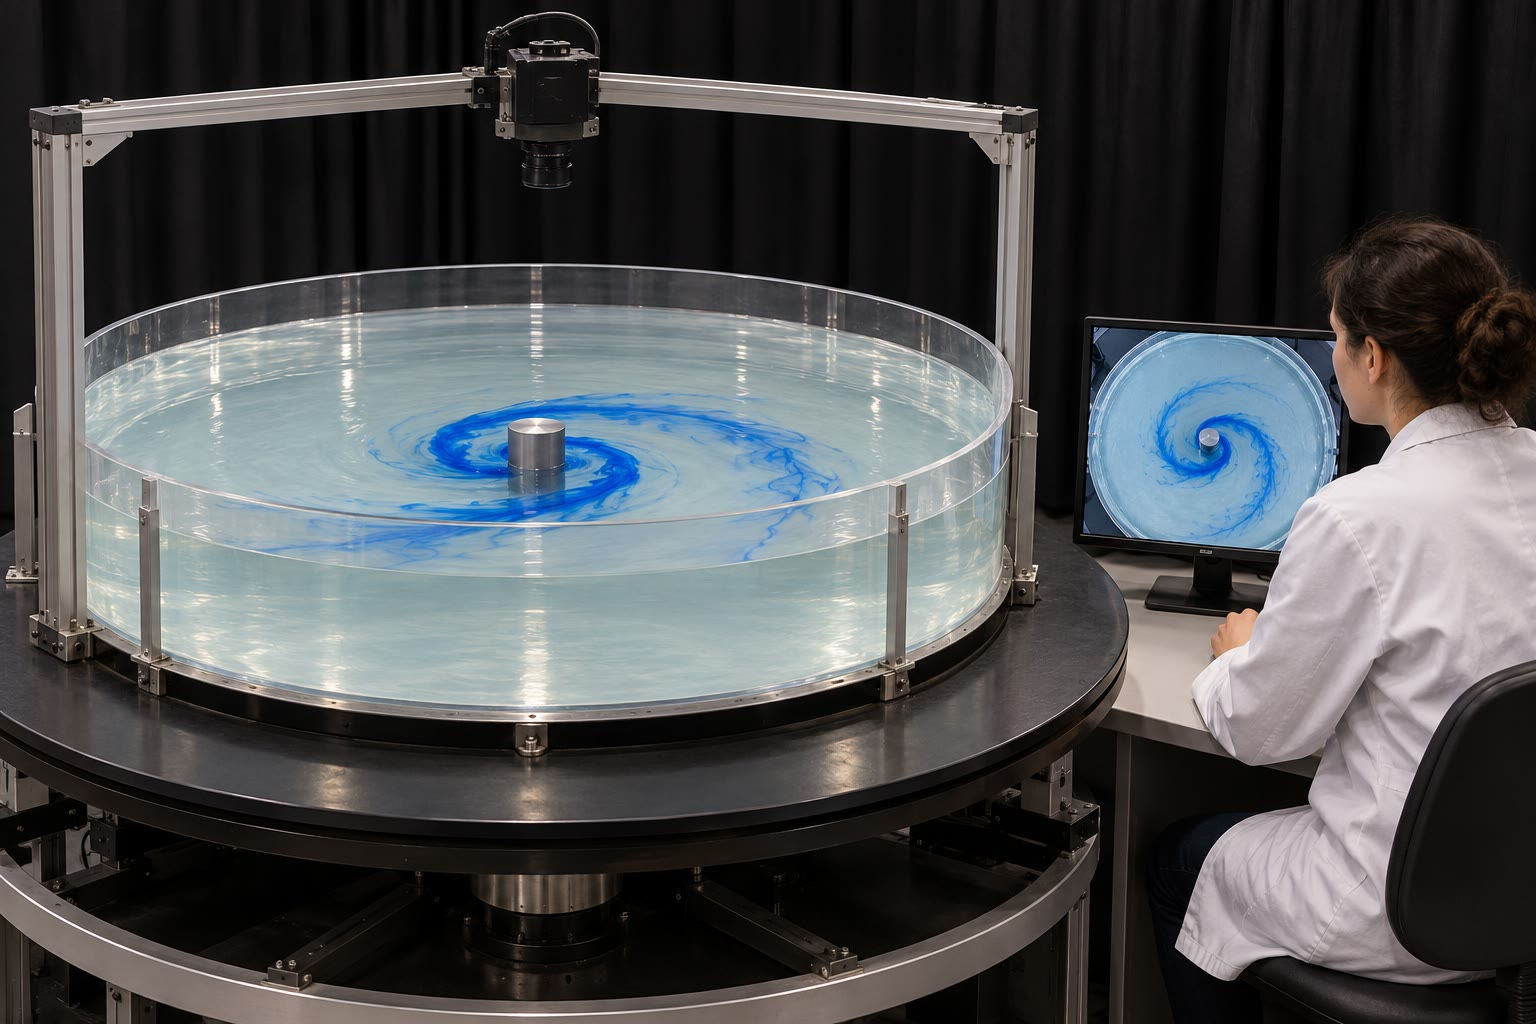
\includegraphics[width=\linewidth]{images/book5/ai/b3-rotating-tank.jpg}

{\scriptsize Un bac en rotation~: un colorant s'enroulant autour d'un cylindre, filmé par une
caméra qui tourne avec la platine (Illustration générée par IA.)}
\end{minipage}
\end{inthelab}

\section{Exercices}

\begin{exercise}[$\star$]\label{exo:b3:gfd-foundations:1}
Prendre $\Omega = \qty{7.292115e-5}{rad/s}$. (a)~Calculer le paramètre de Coriolis et la
période d'inertie à \ang{30}, \ang{45} et \ang{60}~N.
(b)~Calculer le rayon du cercle d'inertie d'un courant de
\qty{0.20}{m/s} à ces mêmes latitudes. (c)~Comparer la période d'inertie à
\ang{30} avec le jour sidéral, \qty{23.9345}{h}.
\end{exercise}

\begin{exercise}[$\star$]\label{exo:b3:gfd-foundations:2}
À \ang{45}~N, calculer le \omterm{def:b3:gfd-foundations:numbers}{nombre de Rossby} d'un tourbillon de poussière (\qty{10}{m/s},
\qty{10}{m}), d'une brise de mer (\qty{5}{m/s}, \qty{20}{km}), d'une dépression
(\qty{15}{m/s}, \qty{1000}{km}) et d'un gyre océanique (\qty{0.05}{m/s},
\qty{2000}{km}). Lesquels sont proches de l'équilibre géostrophique~?
\end{exercise}

\begin{exercise}[$\star$]\label{exo:b3:gfd-foundations:3}
À \ang{45}~N, la température moyenne de la troposphère, \qty{250}{K}, décroît vers
le nord de \qty{5}{K} par \qty{1000}{km}. En utilisant le premier terme
du \omterm{thm:b3:gfd-foundations:thermal-wind}{vent thermique} en altitude, calculer le cisaillement vertical du vent d'ouest et
l'augmentation du vent sur \qty{10}{km}.
\end{exercise}

\begin{exercise}[$\star$]\label{exo:b3:gfd-foundations:4}
La stabilité $E = -(1/\rho)\,\mathrm d\rho_\theta/\mathrm dz$ du kilomètre supérieur
de l'océan se situe entre \num{50e-8} et \qty{1000e-8}{m^{-1}}~;
dans les fosses profondes, elle vaut \qty{e-8}{m^{-1}}. Calculer $N = \sqrt{gE}$, la
période de l'oscillation de flottabilité et $N$ en cycles par heure pour ces
trois valeurs.
\end{exercise}

\begin{exercise}[$\star\star$]\label{exo:b3:gfd-foundations:5}
Un système météorologique a $U = \qty{10}{m/s}$, $L = \qty{1000}{km}$, $H =
\qty{10}{km}$, à \ang{45}~N. (a)~Estimer sa vitesse verticale et son
accélération verticale, et comparer cette dernière à $g$ et au
gradient vertical de la perturbation de pression, $fUL/H$. (b)~Calculer le
terme de Coriolis négligé $\tilde fu$ et le comparer à $g$.
\end{exercise}

\begin{exercise}[$\star\star$]\label{exo:b3:gfd-foundations:6}
Prendre $f = \qty{e-4}{s^{-1}}$ et des isobares circulaires de rayon
\qty{300}{km}. (a)~Le gradient de pression autour d'une dépression donne $V_g =
\qty{20}{m/s}$~: calculer le \omterm{def:b3:gfd-foundations:gradient}{vent du gradient}. (b)~Autour d'un anticyclone,
$V_g = \qty{5}{m/s}$~: calculer le \omterm{def:b3:gfd-foundations:gradient}{vent du gradient}. (c)~Quelle est la plus grande
valeur possible de $V_g$ autour de l'anticyclone, et quel est alors le vent~?
\end{exercise}

\begin{exercise}[$\star\star$]\label{exo:b3:gfd-foundations:7}
Une cuve de \qty{20}{cm} de profondeur tourne une fois toutes les \qty{6}{s}~; son eau a $\nu =
\qty{e-6}{m^2/s}$. (a)~Calculer $f = 2\Omega$, puis le \omterm{def:b3:gfd-foundations:numbers}{nombre de Rossby}
d'un écoulement de \qty{1}{cm/s} autour d'un cylindre de \qty{5}{cm} de large, et le \omterm{def:b3:gfd-foundations:numbers}{nombre
d'Ekman} de la cuve. Une \omterm{thm:b3:gfd-foundations:taylor-proudman}{colonne de Taylor} va-t-elle se former~? (b)~La théorie donne un temps de
mise à l'équilibre $H/\sqrt{\nu\Omega}$~: le calculer en minutes et en tours de la platine.
\end{exercise}

\begin{exercise}[$\star\star$]\label{exo:b3:gfd-foundations:8}
Dans la moyenne zonale de janvier 1991--2020, le vent d'ouest vaut \qty{4.27}{m/s}
à \qty{850}{hPa} et \qty{40.39}{m/s} à \qty{250}{hPa}, à \ang{30}~N,
\qty{5.99}{m/s} et \qty{23.17}{m/s} à \ang{45}~N. Avec $R =
\qty{286.9}{J.kg^{-1}.K^{-1}}$, calculer le gradient méridien de la
température moyenne de la couche aux deux latitudes, et dire pourquoi le courant-jet est plus fort
à \ang{30}~N.
\end{exercise}

\begin{exercise}[$\star\star$]\label{exo:b3:gfd-foundations:9}
(a)~Calculer le \omterm{def:b3:gfd-foundations:rossby-radius}{rayon de déformation de Rossby} de la troposphère ($N =
\qty{0.0113}{s^{-1}}$, $H = \qty{11}{km}$, \ang{45}~N) et de la couche supérieure
de l'océan ($N = \qty{0.00357}{s^{-1}}$, $H = \qty{1000}{m}$, \ang{40.5}~N).
(b)~Avec $a = \qty{6371}{km}$, calculer $\beta$ aux deux latitudes et la
variation relative $\beta L_R/f$ du paramètre de Coriolis sur chaque rayon.
\end{exercise}

\begin{exercise}[$\star\star\star$]\label{exo:b3:gfd-foundations:10}
Une parcelle d'eau de surface animée d'une vitesse $U$ est ralentie par un
frottement linéaire~: $\mathrm du/\mathrm dt = fv - ru$, $\mathrm dv/\mathrm dt = -fu -
rv$. (a)~Résoudre avec $w = u + \mathrm iv$ et décrire la trajectoire. (b)~La
parcelle est aussi entraînée par un courant stationnaire $u_0$ vers l'est~: donner sa
position. (c)~À \ang{45}~N avec $U = \qty{0.2}{m/s}$, $r^{-1} =
\num{4}~\text{jours}$ et $u_0 = \qty{0.05}{m/s}$, donner sa vitesse par rapport au
courant après quatre jours, ainsi que la distance parcourue par dérive.
\end{exercise}

\begin{exercise}[$\star\star\star$]\label{exo:b3:gfd-foundations:11}
À travers un front océanique à \ang{40}~N, la masse volumique de l'eau augmente
vers le nord de \qty{1}{kg/m^3} sur \qty{100}{km}, dans la couche
supérieure de \qty{1000}{m}~; en dessous, l'eau est uniforme et immobile. Avec $\rho_0 =
\qty{1025}{kg/m^3}$, calculer le cisaillement vertical du courant et le
courant en surface. Dans quel sens circule-t-il~?
\end{exercise}

\begin{exercise}[$\star\star\star$]\label{exo:b3:gfd-foundations:12}
La colonne moyenne annuelle à \ang{40.5} N, \ang{30.5} O présente des densités potentielles
$\sigma_\theta = \rho_\theta - \qty{1000}{kg/m^3}$ de 26.029 à
la surface, 26.697 à \qty{100}{m}, 27.079 à \qty{500}{m} et 27.628 à
\qty{1000}{m}. (a)~Calculer $N$ dans chacune des trois couches, en
\unit{s^{-1}} et en cycles par heure. (b)~Quelle couche est la plus
stable, et pourquoi~? (c)~Comparer ces valeurs à la plage de l'océan supérieur
dans l'\cref{exo:b3:gfd-foundations:4}.
\end{exercise}
% ledger: geod5:grs80-defining, earth:Trot, stewart:stability, data:b5-ncep-uwnd, data:b5-woa23-atlantic, earth:Rmean

\section{Problème~: Vents sur la steppe d'Orrin}

\begin{problem}[{Problème du week-end --- la rotation, la stratification et
les vents d'une plaine imaginaire à \ang{48} N}]
\label{pb:b3:gfd-foundations:1}
La steppe d'Orrin est une plaine plate à \ang{48} N, avec un lac, le lac Orrin,
large de \qty{12}{km}, et un petit laboratoire doté d'une cuve en rotation. Prendre
$\Omega = \qty{7.292115e-5}{rad/s}$, $g = \qty{9.81}{m/s^2}$, $R =
\qty{286.9}{J.kg^{-1}.K^{-1}}$ et $c_p = \qty{1004}{J.kg^{-1}.K^{-1}}$.
Toutes les valeurs de la steppe, de son lac et de ses vents sont imaginaires.

\medskip\noindent\textbf{Partie I --- La rotation joue-t-elle un rôle~?}
\begin{enumerate}
\item Calculer le paramètre de Coriolis et la période d'inertie à Orrin.
\item Calculer le \omterm{def:b3:gfd-foundations:numbers}{nombre de Rossby} de cinq écoulements~: l'eau qui s'écoule
  d'une baignoire (\qty{0.1}{m/s} sur \qty{0.3}{m})~; la cuve du laboratoire, qui
  tourne une fois toutes les \qty{10}{s} (avec $f = 2\Omega_{\text{cuve}}$~;
  \qty{5}{mm/s} sur \qty{0.2}{m})~; la brise du soir sur le lac (\qty{5}{m/s},
  \qty{20}{km})~; une dépression (\qty{15}{m/s}, \qty{1000}{km})~; le gyre
  d'un bassin océanique à la même latitude (\qty{0.05}{m/s}, \qty{2000}{km}).
\item Lesquels de ces écoulements ressentent la rotation qui les entraîne, et
  lesquels sont proches de l'équilibre géostrophique~?
\item Calculer le \omterm{def:b3:gfd-foundations:numbers}{nombre d'Ekman} de la cuve (\qty{0.2}{m} de profondeur, $\nu =
  \qty{e-6}{m^2/s}$), de la dépression (viscosité turbulente \qty{10}{m^2/s},
  de profondeur \qty{10}{km}) et du gyre (viscosité turbulente \qty{e-3}{m^2/s},
  de profondeur \qty{1000}{m}).
\item La couche d'Ekman a pour épaisseur $\delta = \sqrt{2\nu/f}$. Montrer que
  $\delta/H = \sqrt{2\,\mathrm{Ek}}$ et calculer $\delta$ pour la cuve et pour
  l'air de la steppe.
\item Que nous disent ces nombres sur les endroits où le frottement joue un rôle~?
\end{enumerate}

\medskip\noindent\textbf{Partie II --- Le vent au sol.}
\begin{enumerate}[resume]
\item Au sol, la pression vaut \qty{1012.9}{hPa} et la température
  \qty{288.1}{K}. Calculer la masse volumique de l'air.
\item La pression au niveau de la mer diminue vers le nord de \qty{4}{hPa} par
  \qty{300}{km}. Calculer le vent géostrophique et donner sa direction.
\item Ce même gradient entoure une dépression dont les isobares ont un rayon
  de \qty{600}{km}. Calculer le \omterm{def:b3:gfd-foundations:numbers}{nombre de Rossby} des isobares et le \omterm{def:b3:gfd-foundations:gradient}{vent
  du gradient}.
\item Ce même gradient entoure un anticyclone de même rayon.
  Calculer le \omterm{def:b3:gfd-foundations:gradient}{vent du gradient}, ainsi que le plus fort gradient de pression, en
  \unit{hPa} par \qty{300}{km}, que l'anticyclone peut supporter.
\end{enumerate}

\medskip\noindent\textbf{Partie III --- Stratification.}
\begin{enumerate}[resume]
\item La température de la troposphère diminue de \qty{6.49}{K/km}.
  Calculer le gradient adiabatique sec $g/c_p$, ainsi que $N$ et la période de
  l'oscillation de flottabilité à \qty{5}{km}, où la température vaut
  \qty{255.7}{K}.
\item Au-dessus de \qty{11}{km}, l'air est isotherme à \qty{216.6}{K}. Montrer que
  $N^2 = g^2/(c_pT)$ à cet endroit, et calculer $N$ ainsi que son rapport à la valeur de
  la question~11.
\item Calculer le \omterm{def:b3:gfd-foundations:rossby-radius}{rayon de déformation de Rossby} de la troposphère d'Orrin, avec le $N$ de
  la question~11 et $H = \qty{10}{km}$, et le comparer à la taille de la
  dépression de la partie~I.
\item En été, les \qty{20}{m} supérieurs du lac Orrin sont plus légers que
  l'eau profonde de \qty{1.5}{kg/m^3} ($\rho_0 = \qty{1000}{kg/m^3}$). Calculer
  la gravité réduite $g' = g\,\Delta\rho/\rho_0$, la vitesse $\sqrt{g'h}$ des
  ondes internes lentes de la couche supérieure, ainsi que le \omterm{def:b3:gfd-foundations:rossby-radius}{rayon de déformation de Rossby}
  $\sqrt{g'h}/f$.
\item La rotation de la Terre va-t-elle façonner les mouvements internes du lac~?
\end{enumerate}

\medskip\noindent\textbf{Partie IV --- Le vent thermique.}
\begin{enumerate}[resume]
\item Deux stations de radiosondage sont distantes de \qty{600}{km} sur un même
  méridien. La température moyenne de la couche comprise entre le sol,
  \qty{1013}{hPa}, et \qty{265}{hPa}, soit environ \qty{10}{km}, vaut \qty{253.0}{K}
  à la station sud et \qty{249.4}{K} à la station nord. Calculer le
  gradient méridien de température en \unit{K} par \qty{1000}{km}.
\item L'épaisseur d'une couche entre deux pressions est $\Delta z = (R\bar
  T/g)\ln(p_b/p_t)$. La calculer aux deux stations, ainsi que la pente de la
  surface à \qty{265}{hPa} par rapport à celle du niveau du sol.
\item En déduire l'augmentation du vent géostrophique entre le sol et
  \qty{265}{hPa}, à partir de cette pente.
\item Calculer la même augmentation à l'aide du théorème du \omterm{thm:b3:gfd-foundations:thermal-wind}{vent thermique} en pression.
\item L'air de la steppe est-il \omterm{def:b3:gfd-foundations:baroclinic}{barotrope} ou \omterm{def:b3:gfd-foundations:baroclinic}{barocline}~? Quel serait le vent
  à \qty{265}{hPa} s'il était \omterm{def:b3:gfd-foundations:baroclinic}{barotrope}~?
\item Calculer l'augmentation à partir du premier terme du \omterm{thm:b3:gfd-foundations:thermal-wind}{vent thermique} en
  hauteur, avec la température moyenne de la troposphère standard entre 0
  et \qty{10}{km}, \qty{255.7}{K}, et comparer.
\item Calculer le vent à \qty{541}{hPa}, soit environ \qty{5}{km}, en supposant que le
  gradient de température est le même à chaque niveau.
\item Le nombre de Richardson $N^2/(\partial u/\partial z)^2$ doit passer sous
  0.25 pour que le cisaillement entretienne la turbulence. Le calculer pour la
  troposphère d'Orrin.
\item En janvier, le vent d'ouest zonal moyen à \qty{250}{hPa} vaut \qty{23.2}{m/s}
  à \ang{45} N et \qty{40.4}{m/s} à \ang{30} N. Comparer avec le vent
  d'Orrin, et expliquer pourquoi un vent local peut dépasser la moyenne zonale.
\item Donner le vent géostrophique à \qty{10}{km} au-dessus de la steppe d'Orrin.
\end{enumerate}
\end{problem}
% ledger: geod5:grs80-defining, stewart:stability, data:b5-ncep-uwnd, nasa:grc-atmos
